\documentclass[DIV12,a4paper]{scrartcl}

\usepackage%[demo]%
{graphicx}
\usepackage[utf8]{inputenc}
\usepackage{listings}
\usepackage{caption}
\usepackage{subcaption}

\graphicspath{ {figures/} }

\newcommand{\defaultwidth}{.8\textwidth}
\newcommand{\halfwidth}{.4\textwidth}


\title{Laboration 2:\\ ASUS Xtion Pro: Calibration, noise characterization and filtering\\{\small Sensors and Sensing}}
\author{Michael Flo{\ss}mann, Anders Wilkstr\"om}
\date{2015--12--07}

\begin{document}
\maketitle

\section{Introduction: Structured light cameras}
Structured light cameras are a low-cost option for depth measuring in three dimensional space. The cameras project a known light pattern to a scene and record the reflection of that light pattern. This recorded data is then used for triangulation.\par
For this lab, the ASUS Xtion Pro sensor was used as a structured light camera.
\section{Task and implementation}
The task at hand was to set up and calibrating the sensor, as well as to characterize the noise in the depth measurement and to set up filtering routines.
\subsection{Basic setup}
To set up the camera, the package \texttt{openni2} for ros-indigo was used. When launching the node \texttt{openni2.launch}, it publishes a wide range of topics from the camera.\par %TODO: Maybe list ALL the topics?
For this laboration, only the topics which publish a viewable image were of interest. This included two main topics:%TODO: Explain the opencv shit

\begin{itemize}
  \item \texttt{/camera/rgb/}\\
    This topic publishes data from the RGB camera on the ASUS Xtion Pro. The topic \texttt{/camera/rgb/raw} shows the unprocessed RGB image like a regular camera. A sample image from this topic is shown in figure \ref{fig:rgb-raw}. %TODO!
  \item \texttt{/camera/depth/}\\
    This topic publishes the depth data as a 2D-array of float variables containing the depth values in meters. A sample image from this topic is shown in figure \ref{fig:depth}.
  \item \texttt{/camera/depth\_registered}\\
    This topic combines the RGB and the depth image into a coloured point cloud. A visualization of this topic through the tool \texttt{rviz} is shown in figure 
\end{itemize}

\begin{figure}
  \centering
  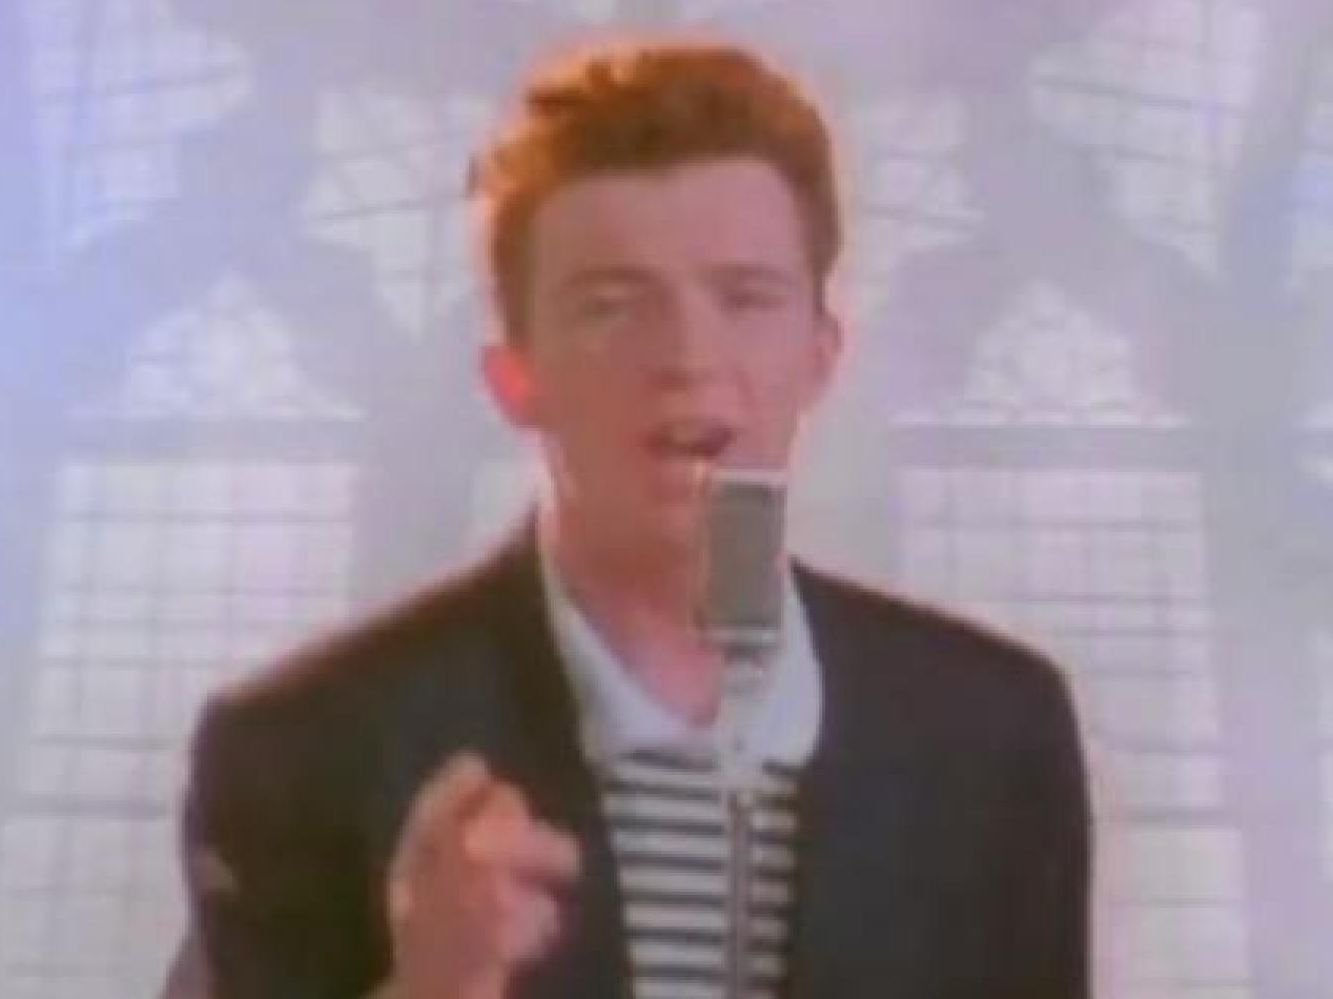
\includegraphics[width=\defaultwidth]{TODO.png}
  \label{fig:rgb-raw}
  \caption{Output image of \texttt{/camera/rgb/raw}}
\end{figure}

\begin{figure}[!htbp]
  \centering
  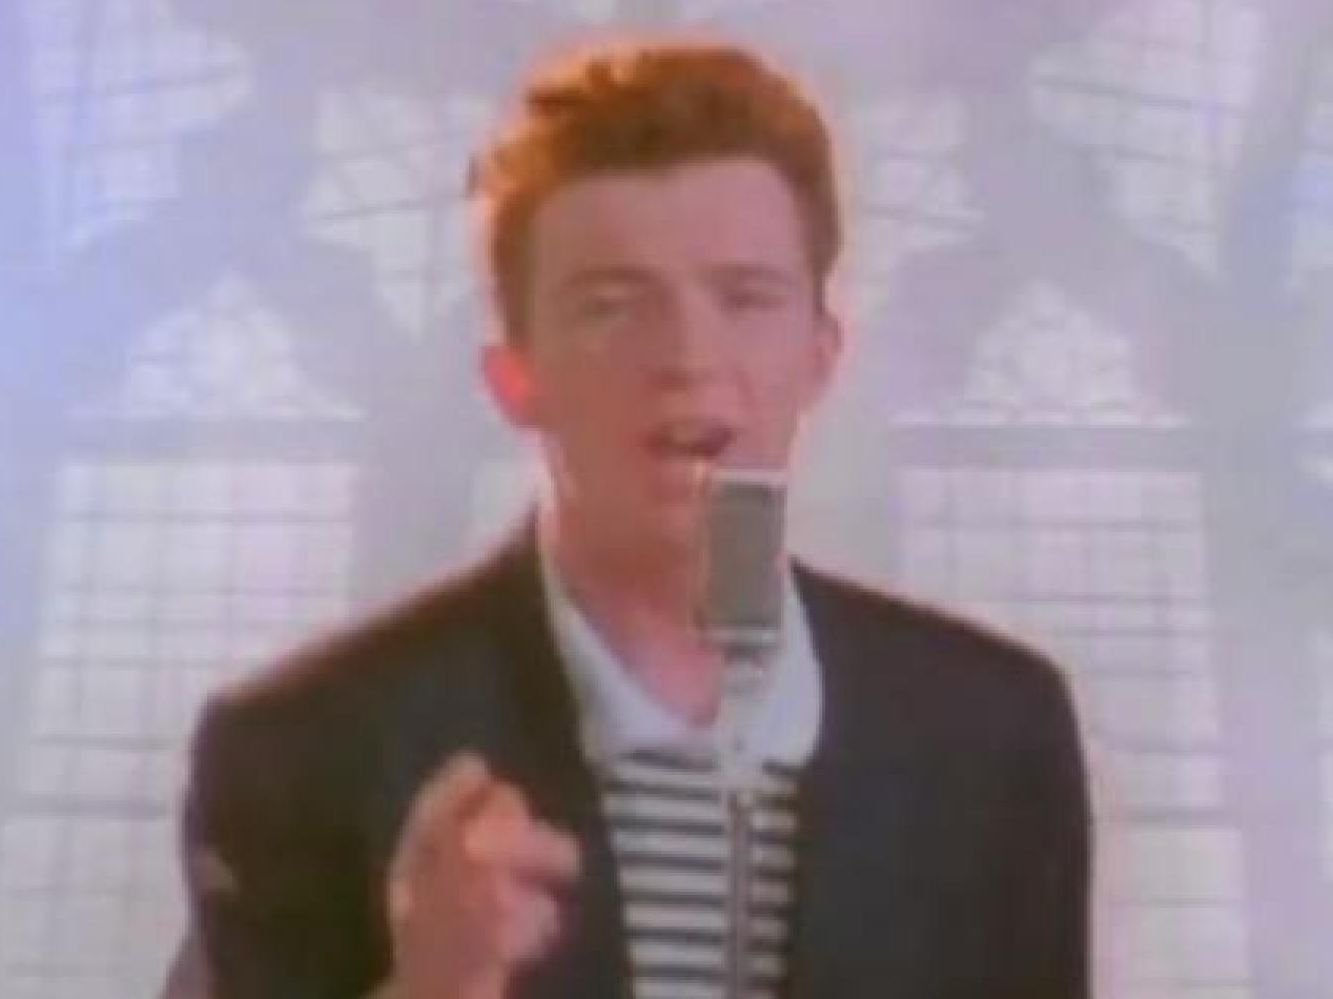
\includegraphics[width=\defaultwidth]{TODO.png}
  \caption{Output image of \texttt{/camera/depth/}}
  \label{fig:depth}
\end{figure}

\begin{figure}[!htbp]
  \centering
  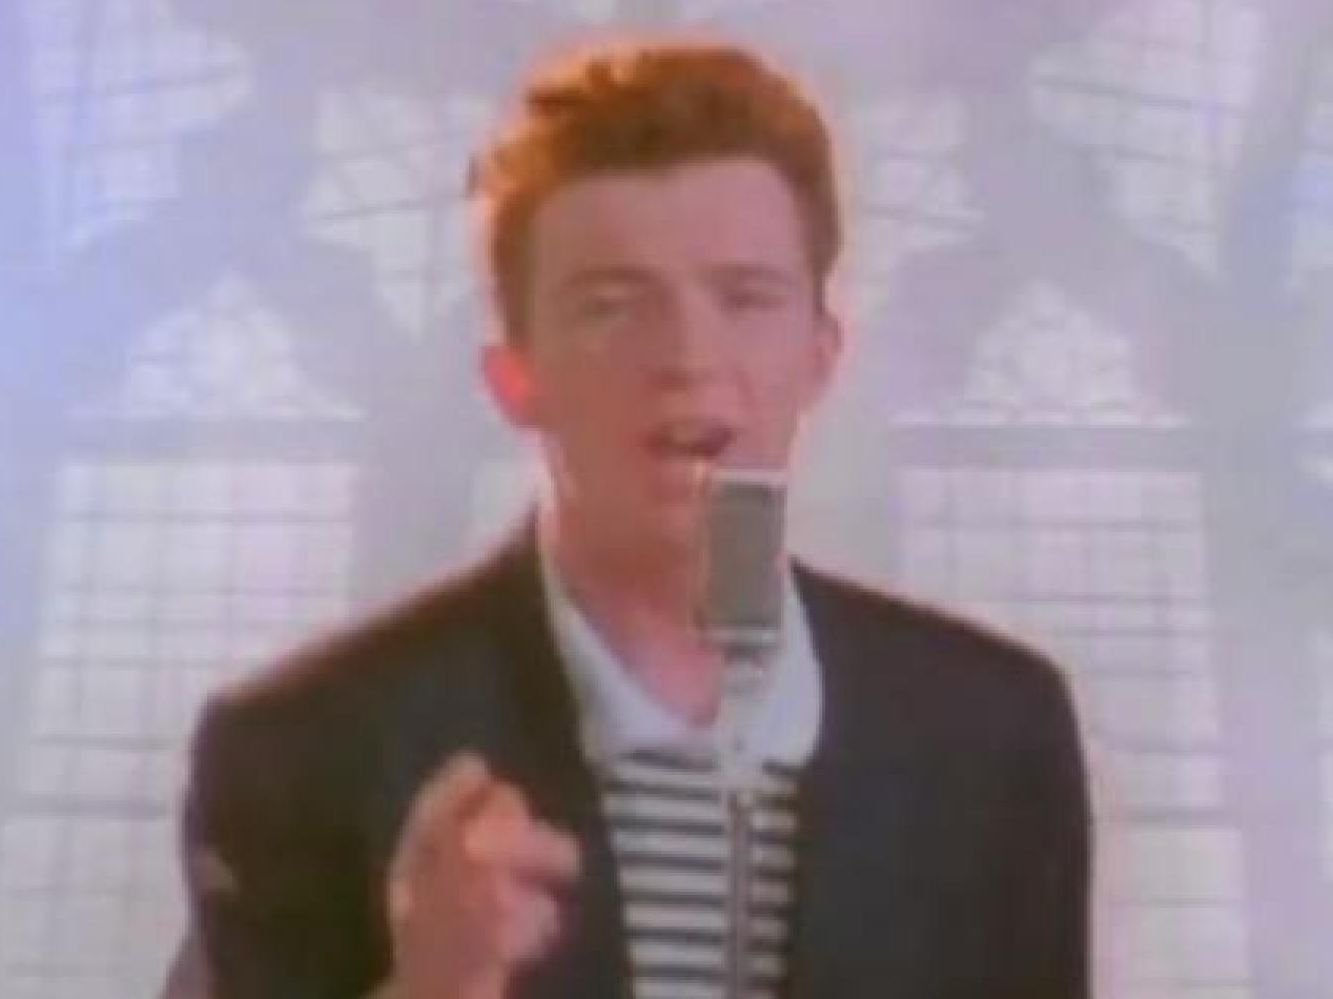
\includegraphics[width=\defaultwidth]{TODO.png}
  \caption{Screenshot of the vizualized pointcloud of \texttt{/camera/depth\_registered}}
  \label{fig:depth_registered}
\end{figure}

\subsection{Basic ROS node}
\label{sec:basic-ros}
After the basic setup, a ROS node template was used as a base to process the images and point clouds published. The received images are shown in figure \ref{fig:rgb-save} and figure \ref{fig:depth-save}.

\begin{figure}[!htbp]
  \centering
  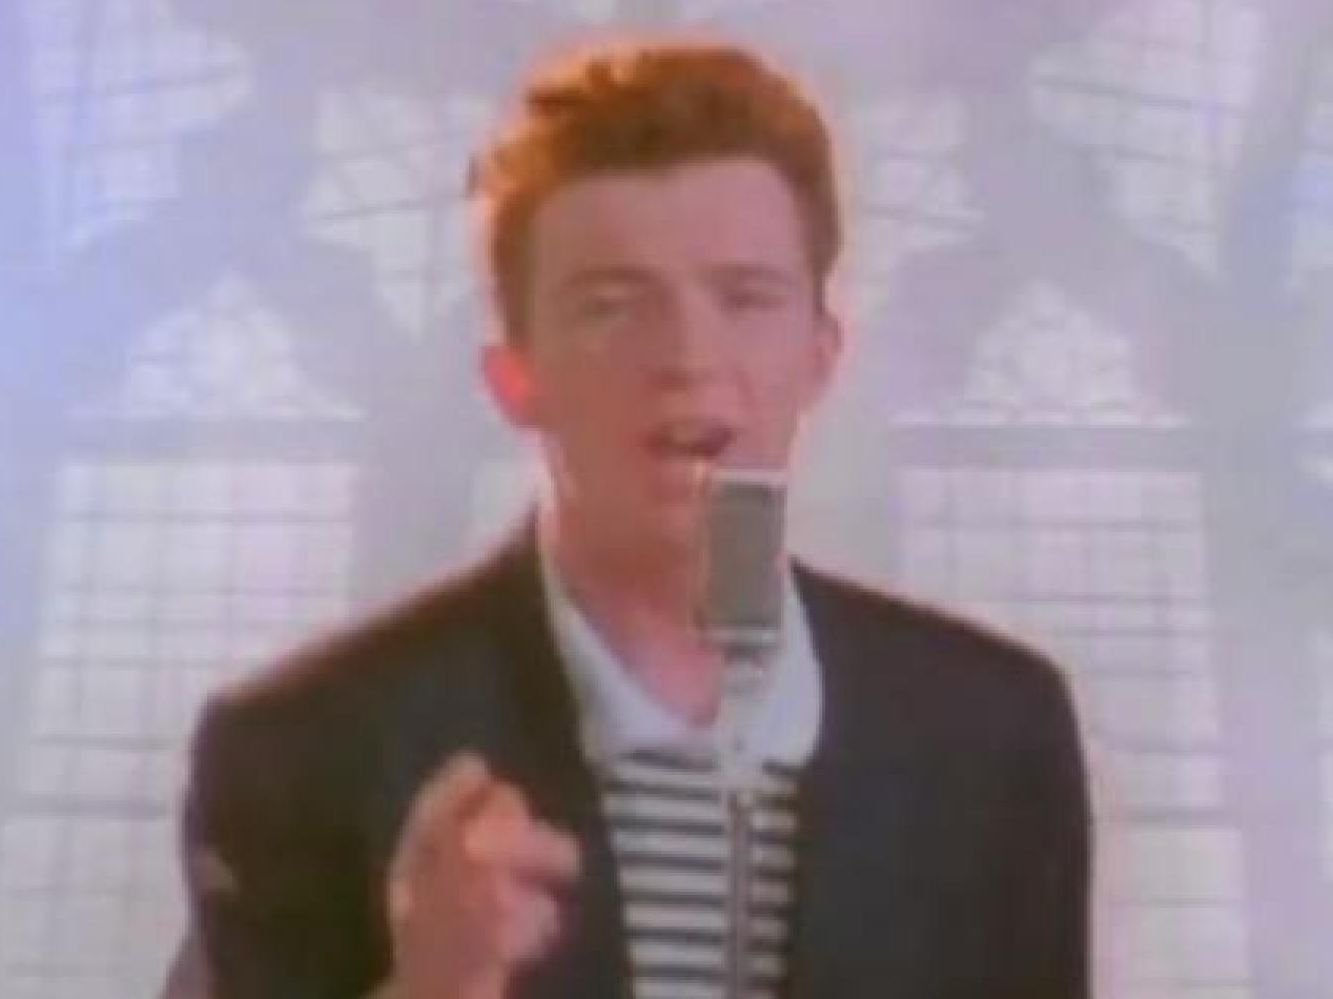
\includegraphics[width=\defaultwidth]{TODO.png}
  \caption{Save of the RGB image}
  \label{fig:rgb-save}
\end{figure}

\begin{figure}[!htbp]
  \centering
  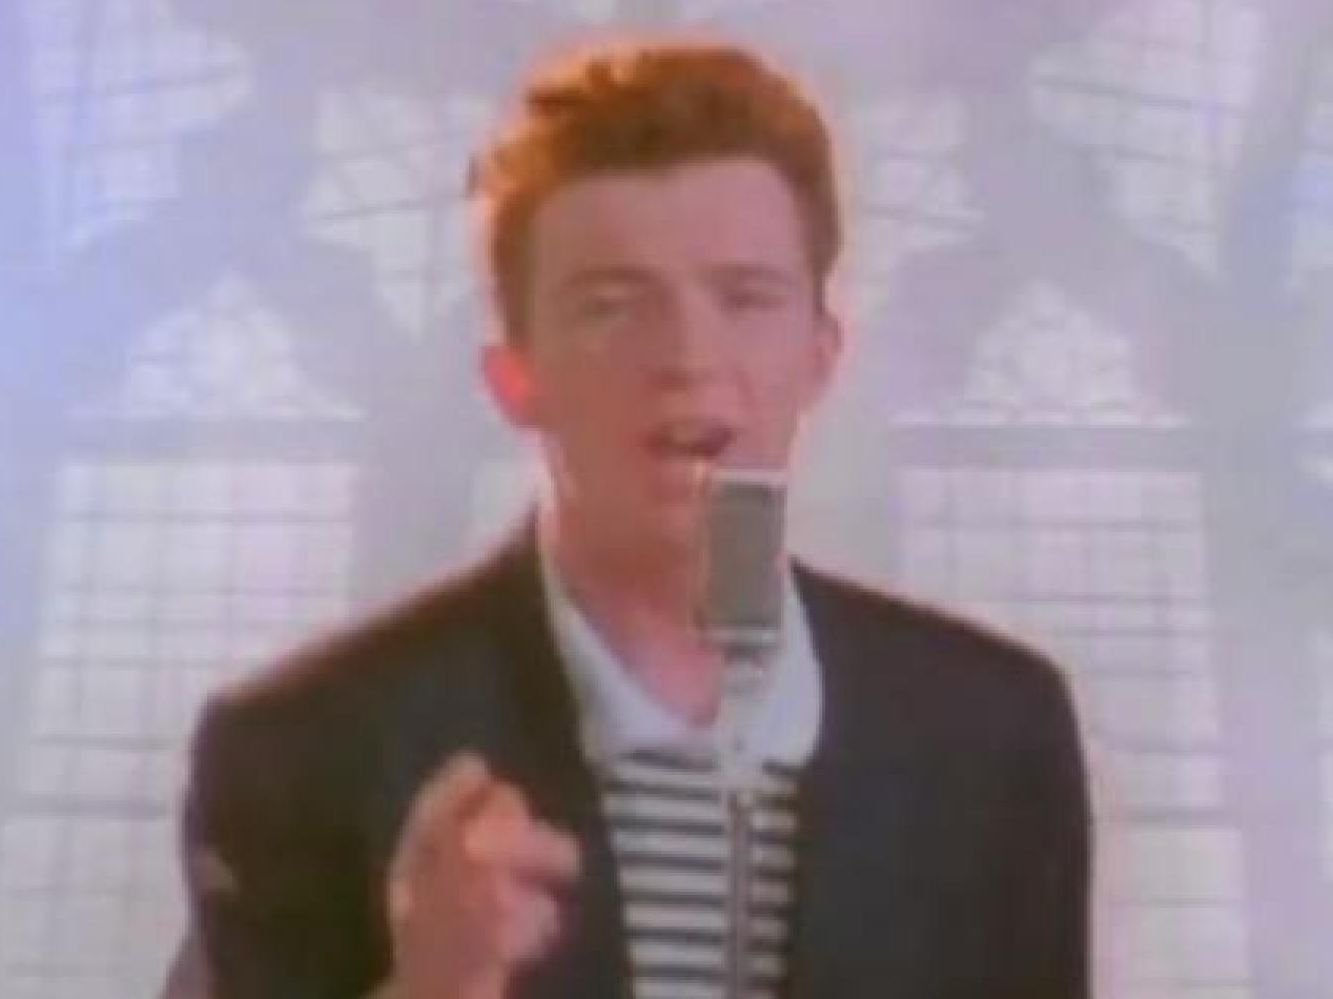
\includegraphics[width=\defaultwidth]{TODO.png}
  \caption{Save of the depth point cloud}
  \label{fig:depth-save}
\end{figure}

\subsection{Color camera calibration}
\label{sec:calibration}

\subsection{Noise characterization}
\label{sec:noise_characterization}

\subsection{Noise filtering}
\label{sec:filtering}
In this part we applied several filters to the depth images in order to remove the noise from the measurement data. These filters are:
\begin{itemize}
\item Gaussian blur
\item Median filtering
\item Bilateral filtering
\item Median over several image samples
\item Average over several image samples
\end{itemize}
The effect on the image data after the application of the filters will be discussed in the following.

\subsubsection{NaN values}
\label{sec:nan}
Whenever the sensor can't evaluate the IR data, the according pixel in the depth image receives a \texttt{NaN} value as the depth value. This can be caused by an object standing too close to the sensor or by IR rays not reaching the sensor due to shadow casting, obstructing objects or scattering. Leaving these \texttt{NaN} values in the image data for processing would negatively influence the filters and thus should to be replaced.\par
Two ways of replacing the \texttt{NaN} values were considered: 
\begin{itemize}
\item Replacing the \texttt{NaN} values with a depth-value of 0.
\item Replacing the \texttt{NaN} values with the last valid pixel scanned.
\end{itemize}
We chose the first method, since the replaced pixels are still identifiable as invalid. Thus, less information is lost.

\subsubsection{Filter effects}
\label{sec:filter_effects}
\begin{figure}[!htbp]
  \centering
  \includegraphics[width=\defaultwidth]{depth_Original.png}
  \caption{Original depth image}
  \label{fig:original_depth}
\end{figure}

\paragraph{Gaussian blur}
\begin{figure}[!htbp]
  \centering
  \includegraphics[width=\defaultwidth]{depth_GaussianBlur.png}
  \caption{Gaussian blur}
  \label{fig:gaussian_blur}
\end{figure}
\paragraph{Median filtering}
\begin{figure}[!htbp]
  \centering
  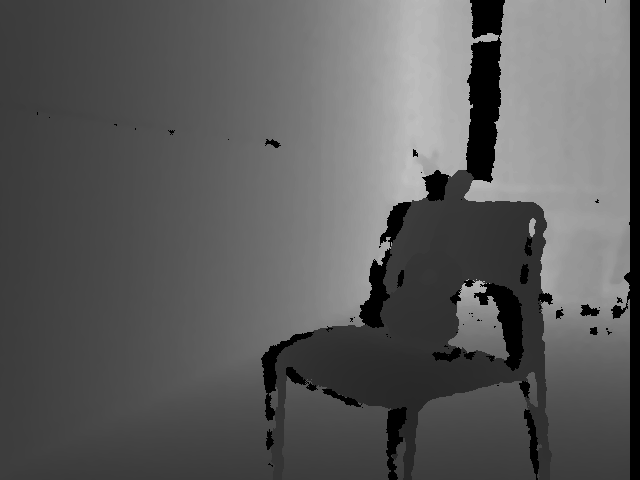
\includegraphics[width=\defaultwidth]{depth_medianBlur.png}
  \caption{Median filtering}
  \label{fig:median_depth}
\end{figure}
\paragraph{Bilateral filtering}
\begin{figure}[!htbp]
  \centering
  \includegraphics[width=\defaultwidth]{depth_bilateral.png}
  \caption{Bilateral filtering}
  \label{fig:bilateral_depth}
\end{figure}
\paragraph{Median over several image samples}
\begin{figure}[!htbp]
  \centering
  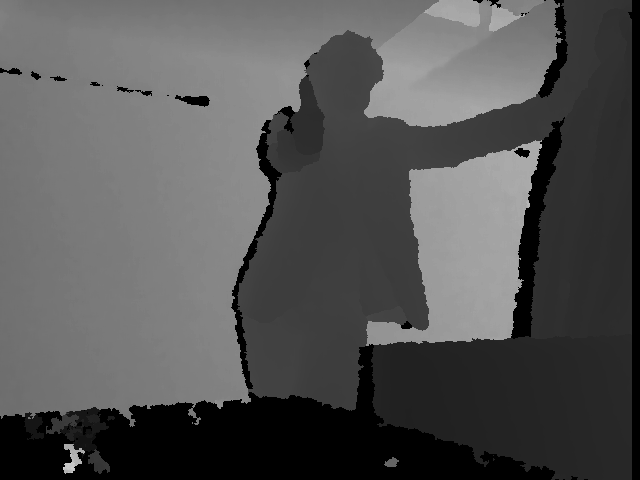
\includegraphics[width=\defaultwidth]{depth_MovingMedianFilter.png}
  \caption{Moving median image}
  \label{fig:moving_median_depth}
\end{figure}
\paragraph{Average over several image samples}
\begin{figure}[!htbp]
  \centering
  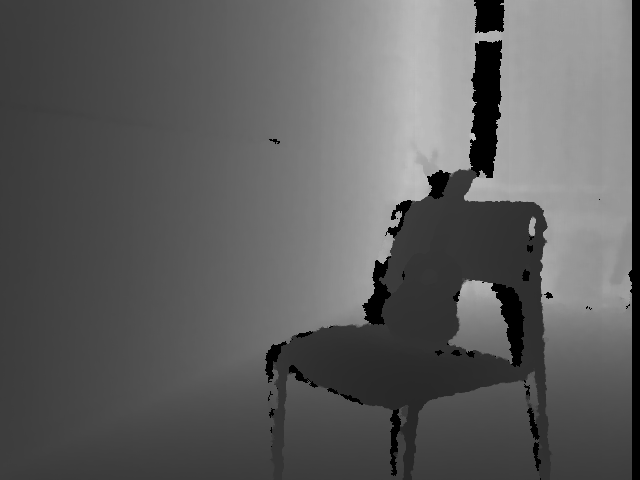
\includegraphics[width=\defaultwidth]{depth_MovingMeanFilter.png}
  \caption{Moving mean image}
  \label{fig:moving_mean_depth}
\end{figure}
\subsubsection{Salt-and-pepper removal properties}
\label{sec:grain_removal}
The depth images didn't suffer from noise visible to the eye. In order to test the noise cancelling properties of the filters, artificial salt-and-pepper noise was added to the image file. This was achieved by changing random pixels in the image to black or white in each received depth-image. %TODO:Listing?
\par
\begin{figure}[!htbp]
  \centering
  \includegraphics[width=\defaultwidth]{depth_Original_spice.png}
  \caption{Original depth image with salt and pepper}
  \label{fig:original_depth_spice}
\end{figure}
\paragraph{Gaussian blur}
\begin{figure}[!htbp]
  \centering
  \includegraphics[width=\defaultwidth]{depth_GaussianBlur_spice.png}
  \caption{Gaussian blur with salt and pepper}
  \label{fig:gaussian_blur}
\end{figure}
\paragraph{Median filtering}
\begin{figure}[!htbp]
  \centering
  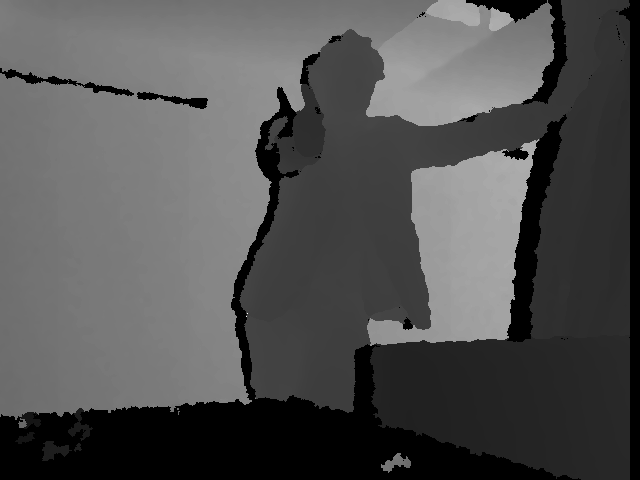
\includegraphics[width=\defaultwidth]{depth_medianBlur_spice.png}
  \caption{Median filtering with salt and pepper}
  \label{fig:median_depth_spice}
\end{figure}
\paragraph{Bilateral filtering}
\begin{figure}[!htbp]
  \centering
  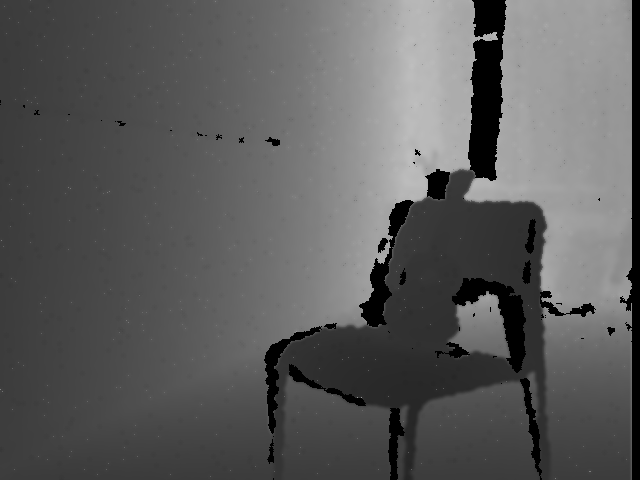
\includegraphics[width=\defaultwidth]{depth_bilateral_spice.png}
  \caption{Bilateral filtering with salt and pepper}
  \label{fig:bilateral_depth_spice}
\end{figure}
\paragraph{Median over several image samples}
\begin{figure}[!htbp]
  \centering
  \includegraphics[width=\defaultwidth]{depth_MovingMedianFilter_spice.png}
  \caption{Moving median image with salt and pepper}
  \label{fig:moving_median_depth_spice}
\end{figure}
\paragraph{Average over several image samples}
\begin{figure}[!htbp]
  \centering
  \includegraphics[width=\defaultwidth]{depth_MovingMeanFilter_spice.png}
  \caption{Moving mean image with salt and pepper}
  \label{fig:moving_mean_depth_spice}
\end{figure}


\end{document}
